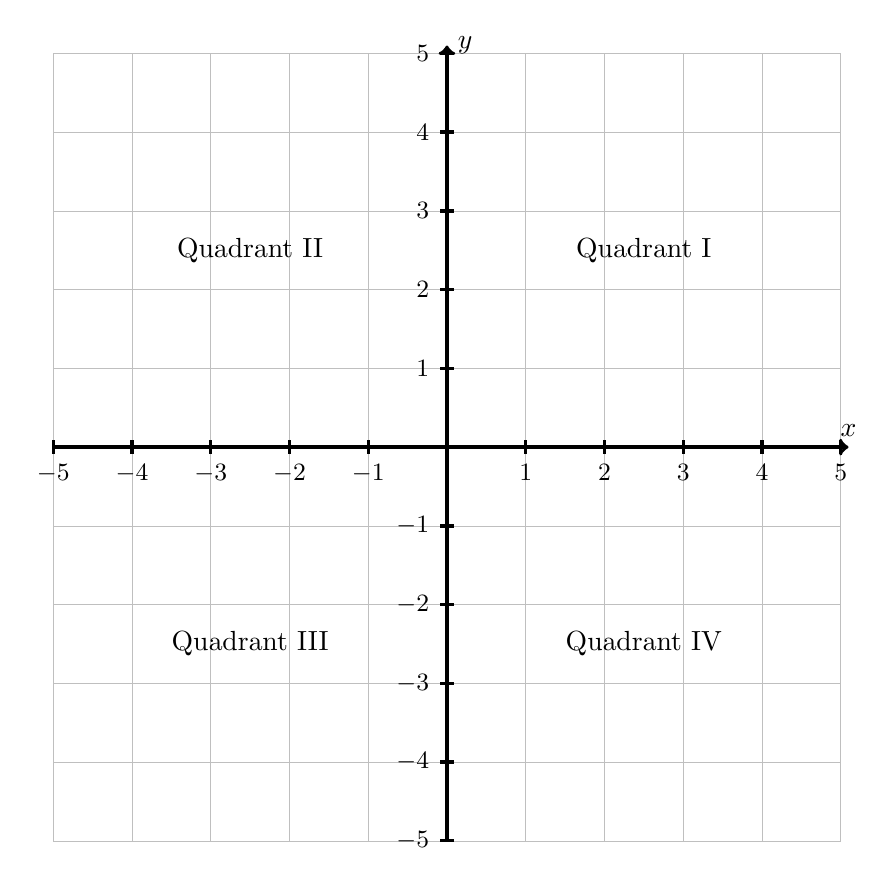
\begin{tikzpicture}
  \def\xmin{-5}
  \def\xmax{5}
  \def\ymin{-5}
  \def\ymax{5}
  \path [draw, help lines, opacity=.5]  (\xmin,\ymin) grid (\xmax,\ymax);
  \foreach \i in {1,...,5} 
  \draw [very thick] (\i,2.5pt) -- +(0,-5pt) node [anchor=north, font=\small] {$\i$}
  (-\i,2.5pt) -- +(0,-5pt) node [anchor=north, font=\small] {$-\i$} 
  (2.5pt,\i) -- +(-5pt,0) node [anchor=east, font=\small] {$\i$}
  (2.5pt,-\i) -- +(-5pt,0) node [anchor=east, font=\small] {$-\i$};
  \draw [very thick,->] (\xmin,0) -- (\xmax+.1,0) node [anchor=south] {$x$};
  \draw [very thick,->] (0,\ymin) -- (0,\ymax+.1) node [anchor=west] {$y$};
  \node at (2.5,2.5) {Quadrant I};
  \node at (-2.5,2.5) {Quadrant II};
  \node at (-2.5,-2.5) {Quadrant III};
  \node at (2.5,-2.5) {Quadrant IV};
\end{tikzpicture}
